\documentclass[11pt,pdftex,a4paper, twocolumn]{article}
\usepackage[ngerman]{babel}
\usepackage[utf8]{inputenc}
\usepackage{url}
\usepackage{float}
\usepackage[pdftex]{graphicx}
\usepackage{listings}
%\usepackage[pdftex]{graphicx}
\include{sort}
\addto\captionsngerman{\renewcommand{\figurename}{Fig.}}
\setlength{\abovecaptionskip}{0mm} 
\setlength{\belowcaptionskip}{0mm} 
\setlength{\dblfloatsep}{0mm} 
\begin{document}
\title{Projekt-INF:\\
Implementation of in-place mergesort algorithms}
\author{Patrick Spaney, Kai Ziegler, Jonas Kittelberger, \\ Raphael Brösamle}
\date{Institut für Formale Methoden der Informatik \\ Universität Stuttgart\\
\normalsize Betreuer: Dr. Armin Weiß\\
Prüfer: Prof. Dr. Volker Diekert}
\maketitle
%%%%%%%%%%%%%%%%%%%%%%%%%%%%%%%%%%%%%%%%%%%%%%%%
%%%%%%%%%%%%%%%%%%%%%%%%%%%%%%%%%%%%%%%%%%%%%%%%
\section*{Introduction}
Traditionally, the problem of sorting a given array by the key values of its elements is a common problem in computer science and thus has been subject to extensive research throughout the evolution of the field. \\
Merge sort is a sorting algorithm that is of special interest due to its $O(n*log(n))$ worst case time bound. Therefore, when a guaranteed worst-case runtime matters, merge sort is chosen over e.g. standard implementations of quicksort, which are usually very fast but have an upper bound of $O(n^{2})$. At the same time, other worst-case efficient sorting algorithms like heapsort are often considerably slower, giving merge sort the edge in many situations. \\
It employs the \textit{“divide and conquer”} paradigm by dividing the given list into smaller sublists, either to a size of one that can always be considered sorted, or until some lower bound is reached, at which point another sorting algorithm is used. Those sorted sublists are then consecutively merged, creating one sorted list from two smaller ones at a time. \\
This allows very simple recursive top-down implementations whose functionality is largely affected by the choice of merging strategies. \\
As one can see, standard versions of merge sort can also be easily parallelised, but this property does not hold for the implementations we will present here because they rely on using not yet sorted parts of the list as extra space to speed up the sorting process. \\
Despite its desirable properties, one big downside of naive merge sort implementations is the required linear extra space, making in-place algorithms like quicksort or heapsort a more suitable choice if memory usage is essential. \\
Therefore, many in-place variants of merge-sorts have been suggested by several authors, ranging from implementations for in-place merges that can then be easily integrated in a naive merge-sort algorithm by replacing the previous merging procedure to entirely modified sorting schemes. \\
In this paper we will discuss a full in-place merge sort by Reinhardt\cite{Reinhardt92} and two in-place merging algorithms, one by Chen\cite{Chen06} and another by Huang and Langston\cite{huang1988practical}. We used the latter ones to implement simple top-down in-place merge sorts. \\
We will describe our implementations giving special attention to parts where our implementation differs from the original algorithms, which applies especially to some versions of Reinhardt’s algorithm. \\
Afterwards, we will give an overview on the various tests we ran, comparing our implementations both against one another and against existing in-place merge sort implementations. We focuse on measuring the performance in means of time, comparisons and assignments. The latter ones are well established measures of complexity for sorting algorithms as they are independent of the machine the algorithm is running on. \\

\section*{Literaturrecherche \"uber in-place Mergesort Algorithmen}
\textbf{TODO: BottomUpHeapSort\cite{wegener1993bottom}.} \\
\textbf{TODO: Armins Paper:\cite{edelkamp2019worst}} \\

\section*{Description of implementations}
\subsection*{Test environment and standard mergesort}
We started by implementing some versions of the standard merge sort with extra storage matching the size of the given list. In the files \textit{rec\_mergesort\_reference.cpp} and \textit{rec\_mergesort\_iter.cpp}, we implemented the recursive standard merge sort on a reference to a vector and on begin-/end-iterators. They work according to the known principle of pairwise merging two lists to one bigger list. Thereby we merge between the extra storage and the original list alternating each iteration. We implemented insertion sort and a small sort which can be used for small sizes in the last recursion step. The last step can be performed within the original list or between the lists so that a final copy of the whole list can be avoided in any case. \\
We also implemented an iterative merge sort (\textit{iterative\_mergesort.cpp}) which similarly needs additional storage the same size of the original list. \\
A disadvantage of the recursive variant is the logarithmic space for the internal stack. But on the other side, it is a simple and elegant way to split a long list into parts of equal length throughout all recursion levels. Thus it is important to remark that true in-place sort algorithms may also use extra space for recursive execution (even though they just work on the original list per definition). \\
For test cases we implemented different test environments. We used the main function in the \textit{“TestAndEvaluation”}-project for obtaining our test results. The user can choose between different types to sort, the list sizes and a lot of other options (\textit{main.h}). The user can start the test by executing the main procedure (\textit{main.cpp}) and the results (average time, comparisons and assignments per size of the list) are written to CSV-Files. We implemented a general BigType (\textit{structs.h}) and a general PointerType to weigh assignments and/or comparisons differently. Sorting the BigType makes the assignments more expensive and the user can choose whether the computation of the comparisons should also be expensive. To get expensive comparisons and cheap assignments, the user can choose the PointerType on the BigType with expensive comparisons.

\subsection*{Reinhardt}
Reinhardt‘s in-place mergesort algorithm consists of two main procedures: \\
In the first step, $\frac{2}{3}$ of the unsorted elements are sorted by using the other $\frac{1}{3}$ of the unsorted elements as gap \textit{(reinhardt\_gapsort)}. \\
In the second step, the sorted elements of the first step (called “short” list) are merged with the previous sorted elements (called “long” list) \textit{(reinhardt\_merge)}. \\
Therefore, we can merge $\frac{2}{3}$ of the unsorted elements into the sorted list in a single iteration. Despite this being a full description of an $O(n*log(n))$ in-place-mergesort, we need a lot of time to swap all elements after one iteration as well as in the asymmetric merge in step two. \\
Therefore, we implemented some improvements, most of them also described in the paper: \\
In the whole algorithm we regard our elements as a ring list to skip the moves after one iteration \textit{(*\_ring)}. For this we “overloaded” the dereference operator so that every iterator points on the shifted element. But because of the worse results and the incompatibility with the following improvements, we just continued without the ring list and leave a more detailed explanation. \\
We also implemented two other procedures that can be executed instead of the “usual” step \textit{(quick\_steps)}. They perform a quickselect- or quicksort-step on the unsorted elements and then merge them with a part of the long list. After this step, the merged elements are on their correct position and do not need to be considered any more. \\
In the following, we give a more detailed description of the stated procedures. \\
$ $ \\
\textbf{In-place mergesort basic routine \textit{(inplace\_mergesort\_[qsel / qsort])}} \\
Firstly, we sort $\frac{4}{5}$ elements of the whole list by using $\frac{1}{5}$ as gap. This is possible in the first iteration because we do not need to consider the gap for step two. After that, we call the recursive procedure which executes the two steps mentioned above. We implemented an integer-flag where the user can choose the frequency of quicksort or quickselect iteration compared to the usual iteration. A quicksort step can leave the new gap on the right side, therefore we needed to implement an analogous second procedure for this case. As soon as the gap size undercuts a short number, we execute one parallel insertion sort step for the left block by use of binary search for efficiency reasons. \\
$ $ \\
\textbf{Step one \textit{(reinhardt\_gapsort)}} \\
We sort the elements between the passed iterators by using $\frac{size}{4}$ elements as a gap on the left or on the right side. For this we firstly sort four quarters of the list with the usual recursive mergesort \textit{(rec\_mergesort\_iter)} and the gap as “extra storage”. Therefore, we permanently have to swap the gap elements instead of just assigning them to the extra memory. \\
Afterwards we merge the four quarters in a way quite similar to the symmetric merge procedure described below (step two). \\
Step one can also be used as a full sorting algorithm with $\frac{size}{4}$ extra space \textit{(reinhardt\_extrasort)}. The number of assignments is obviously bigger for the in-place mergesort due to swapping instead of moving. But $\frac{size}{4}$ extra space is only just enough to avoid any additional costs for swapping or shifting. \\
$ $ \\
\textbf{Step two \textit{(reinhardt\_merge)}} \\
The merge procedure expects the longer list being between the gap and the shorter list and a minimal gap size of half of the shorter list. The merge direction changes after a “collision” with the longer list, exactly as described by Reinhardt\cite{Reinhardt92} (chapter two). \\
To reduce the number of comparisions, we also implemented an asymmetric merge variant. For this we compare the first element of the shorter list with the $2^n$’th element of the longer list whereas $n$ is chosen depending on the relation of the list sizes. Afterwards, the whole block of the longer list can be moved or a binary search in the block is needed. The case $2^n = 1$ is equal to the usual symmetric merge. \\
$ $ \\
\textbf{Quickselect and Quicksort iteration \textit{(quick\_steps)}} \\
The quickselect iteration extracts the $\frac{2}{3}$-smallest element of the gap and partitions the gap elements around. Note that this step should not exceed $O(n*log(n))$ in worst case to retain $O(n*log(n))$ as worst case runtime for the whole sort. Afterwards, the small-elements partition is sorted with step one by using the big-elements partition as gap. Now we determine the fitting small-elements list of the long list by binary search and then the two small-elements lists are merged (after a possibly necessary swap of the lists). \\
Although there is a non-negligible overhead for the quickselect procedure, all the merged elements are on their correct position and the gap size is reduced by the same amount as in the usual step. \\
$ $ \\
The quicksort iteration as described in chapter five does not guarantee a specific reduction of the gap size, but it moves half of the long list to the correct position. Therefore, the size of the remaining “long” list could get very small and in this case we just continue to execute the usual iteration in the basic routine for efficiency reasons. \\
The quicksort step works as follows: \\
After quicksort on the unsorted elements with the middle element of the long list as pivot, we sort the partition of the bigger or the smaller elements depending on the size of the partitions. Before the following merge with the bigger or the smaller half of the long list, we possibly need some swaps to get the lists to be merged in the right order. After the merge, the remaining gap may have changed on the other side and in this case the other recursive basic routine is called.

\subsection*{Chen}
Chen describes a linear time in-place merging procedure that we used to implement a merge sort algorithm. \\
The merge requires two adjacent sorted lists and a block size k as input. Both sublists are divided into a series of blocks, each of size k (with the possible exception of an undersized leftmost block of length f). The two rightmost blocks of the first sublist will initially be used as internal buffers. During the execution of the merge, the order of the left list's blocks may be altered but the elements within each block, again excluding the buffer blocks, remain sorted. The elements are inserted into a hole, which is created by moving one element to some temporary memory. As the algorithm progresses, the hole is always at the position where the next element will be inserted. While the position of the hole and the second list’s smallest element are only incremented by 1 each time they are updated, the buffers and the first list’s current block, containing its smallest elements, require more attention. We will explain this in the following description of the corresponding procedures. \\
We do not provide a detailed description of all the procedures, as our implementation does not differ from the pseudo-code given by Chen in most parts, but we will provide a short overview. \\
Some notations: $n$ denotes the size of the list. As in the original paper we will use X to denote the first and Y to denote the second sublist. \\
$ $ \\
\textbf{\textit{mergesort\_chen}}: \\
Divides the given list into two sublists of equal size. The first sublist is always sorted with another merge sort algorithm, using the second one as extra space, while the second sublist is handled by a recursive call to \textit{“mergesort\_chen”}. The recursion stops when the list contains 50 or less elements and the remaining list is sorted by insertion sort.  Both sublists are then merged using the “merge”-procedure with block size $k=\sqrt{n}$. \\
$ $ \\
\textbf{\textit{merge}}: \\
This is the main procedure of Chen’s merging algorithm. Firstly, there is some preparatory work, mostly initialising variables, like the size $f$ of a possible undersized leftmost block and the position of the $b1$ and $b2$ buffer (specificly the iterators to the respective first element). The buffers initially consist of the two rightmost X-blocks. Also the hole must be created and the corresponding element must be stored in temporary memory. Afterwards, we begin to merge both sublists in a while-loop until there is no more room for the buffers in the remainder of X, i.e. all but 2k X-elements are in their final position. First we check whether the current X- or Y-element is smaller or the second sublist is exhausted, in which case we always pick the X-element. In either case the following moves will be executed: \\
hole $\leftarrow$ smaller $\leftarrow$ buffer element $\leftarrow$ element currently in next hole. \\
While the hole position $z$ and the current Y-element position $y$ are only incremented by one in each iteration, it is a bit trickier to keep $b1$, $b2$ and the current X-element position $x$ updated. The latter one is updated each time it hits a block boundary by the \textit{“findNextXBlock”} procedure. If the hole is not currently positioned in the block just left by $x$, then $b2$ is set to $x-k$ before $x$ is updated because the block does now consist solely of buffer elements. The same buffer-update will be applied if $y$ reaches a block boundary, but we do not need to check for the position of $z$ in this case. Furthermore, $b2$ must be invalidated if the hole enters the current $b2$ block, which is done by setting $b2$ to the end-iterator of the current list. In each iteration we need to increment $b1$ and when it hits a block boundary, we set it to $b2$ if a $b2$ buffer is available. Otherwise the $b1$ buffer can be reused and we set it to $b1-k$. After the while-loop terminates, we can put the element we used to create the initial hole back in the current hole, which is the first position of the remaining buffer. \\
This process leaves us with a sorted output block where every element is already in its final position, two unsorted buffer blocks and possibly a sorted remainder of Y. \\
As suggested by Chen, we handled the remaining list by first sorting the buffer, merging the sorted buffer and the remaining Y-elements with block size $\sqrt{k}$ and then using \textit{“mergeBandY”} in the recursive invocation of \textit{“merge”}. The proposed heapsort for sorting the buffer is replaced by our \textit{“mergesort\_chen”} procedure, as our goal is to compare different in-place merge sort algorithms without using other sorting algorithms for greater parts of the lists. Moreover, due to the $O(k^{2}+|remainder of Y|)$ time complexity of \textit{“mergeBandY”}, we do the recursive step two times instead of one before using \textit{“mergeBandY”} because the list can still be quite large in the first recursion step. \\
$ $ \\
\textbf{\textit{mergeBandY}}: \\
Merges an unsorted block B with a sorted Block Y until B or Y is exhausted. \\
If B is exhausted first, the merge is finished, otherwise the remaining B-elements need to be sorted differently. Again, we chose \textit{“mergesort\_chen”} over heapsort for this task. \\
This procedure is not very efficient because in each step we determine the smallest remaining B-element and compare it with the current Y-element. \\
$ $ \\
\textbf{\textit{findNextXBlock}}: \\
As the X-blocks are not always in their correct order during the merging process, we use this function to determine the next block after we hit a block boundary. \\
This is accomplished by comparing all X-blocks, excluding buffer blocks, by their respective first and last element and choosing the X-block with the smallest elements.

\subsection*{Huang and Langston}
Like Chen, Huang and Langston describe a linear time in-place merging procedure that can then be used to implement a full merge sort algorithm. \\
The merge is accomplished by moving the $\sqrt{n}$ largest elements of the list to the front and using them as internal buffer.
The remainder of each sublist is then divided into blocks of size $\sqrt{n}$. In case this is not possible without at least one undersized block we must do some preparatory work first. \\
We omit the details here and assume the list is ready for the main algorithm to commence. \\
First, the blocks need to be sorted by their rightmost elements. \\
Selection sort is a good choice for this as it is very easy to implement and performs only $O(n)$ swaps. \\
Afterwards we need to determine the next two series of elements to be merged. \\
The first series consists of the first block after the buffer and all following blocks until one block’s rightmost element is larger than the next block’s leftmost element. The second series consists only of the latter block. These two series are merged, beginning at the leftmost buffer position and breaking ties in favour of the first series until the first series is exhausted. Therefore, the second series will still contain at least one element and the buffer elements will be back in one piece, adjacent to the left of the second series’ remainder.
This process, starting with finding the two series, is now repeated with the first “block” of the new first series being the remainder of the last second series until there is no second series to be found. \\
Then we just need to perform a cyclic shift of the remaining elements and the buffer, leaving the list sorted except for its $\sqrt{n}$ rightmost elements, consisting only of the buffer elements. Since these are the largest elements of the list, we just need to sort them in order to finish sorting the whole list. \\
The paper of Huang and Langston does not provide a specific suggestion as to how the buffer should be sorted. For the purpose of using solely the algorithm in the paper, we sort the buffer by a recursive call to our merge sort implemented with the described merge of Huang and Langston. \\
$ $ \\
We will give a quick outline of our implementation’s basic procedures. \\
Note that $n$ is always referring to the size of the list \textit{“merge”} is initially called with. \\
$ $ \\
\textbf{\textit{mergesort}}: \\
Divides the given list into two sublists of equal size. The first sublist is always sorted with another merge sort algorithm, using the second one as extra space, while the second sublist is handled by a recursive call to \textit{“mergesort”}. The recursion stops when the list contains 50 or less elements and the remaining list is sorted by insertion sort.  Both sublists are then merged using the \textit{“merge”}-procedure. \\
$ $ \\
\textbf{\textit{merge}}: \\
Determines the $\sqrt{n}$ largest elements that will constitute the buffer and whether the remaining sublists meet the size requirements (integral multiples of $\sqrt{n}$). If the requirements are met, the basic merge procedure, as described above, can commence. The buffer will then be extracted using two cyclic shifts and \textit{“basic\_inplace\_merge”} is called. Otherwise some undersized blocks must be extracted alongside the buffer, so we can again use \textit{“basic\_inplace\_merge”} on the remaining list (and merge one of the undersized blocks afterwards). \\
$ $ \\
\textbf{\textit{basic\_inplace\_merge}}: \\
This is where the actual merging begins. As explained above, we now regard our list, excluding the buffer, as a list of blocks, each of size $\sqrt{n}$. The blocks need first be sorted by their rightmost element. This is done by \textit{“sort\_blocks”}, which is essentially an implementation of selection sort. The following process of finding new series and merging them is accomplished by alternating calls to \textit{“merge\_with\_buffer”} and \textit{“find\_series”}, the first one obviously performing the merge and returning the start of the new first series. The latter one simply returns the start of the new second series or, if no such series can be found, the end-iterator that serves as condition to terminate the loop. Afterwards, the buffer is shifted to its final place and is sorted. This is done by using \textit{“mergesort”}, for the purpose of testing only the merge of Huang and Langston. \\
$ $ \\
\textbf{\textit{merge\_with\_buffer}}: \\
Merges the first and second series, with the resulting list beginning at the first buffer position, until the first series’ elements are exhausted. Ties are broken in favour of the first series. As a result, the buffer will be in one place after the procedure, adjacent to the right of the sorted list and followed by at least one unmerged element of the second series.

\section*{Test results}
In the following we will describe and analyse the results of the tests. Although it is not possible to compare all versions of the in-place merge sorts with all possible test conditions, we try to cover a broad range to figure out the main points. The raw data and further results are given in the “Test\_Diagramme” file \\
For all the tests given here, we sorted equally distributed integer values in multiple runs (of course more runs for smaller lists) on the server. We start by comparing our in-place merge sort implementations between each other. \\
\begin{figure}[H]
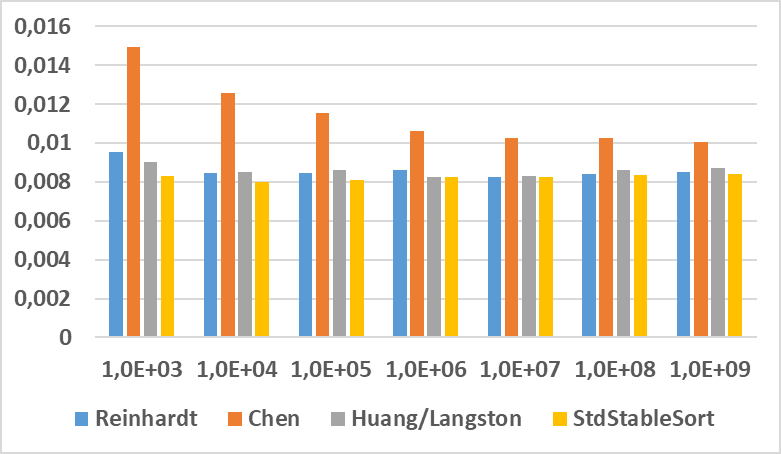
\includegraphics[width=\linewidth]{Diagramm-Bilder/ints-time.JPG} \\
\caption{ $ \frac{Time}{n*log(n)} $ for different integer list sizes $ n $ } \label{fig:ints-time}
\end{figure}
Integers do not need much time to be assigned. Therefore the time in this test is mainly influenced by other statements like index computations. This can also be seen by a comparison with the following result. \\
\begin{figure}[H]
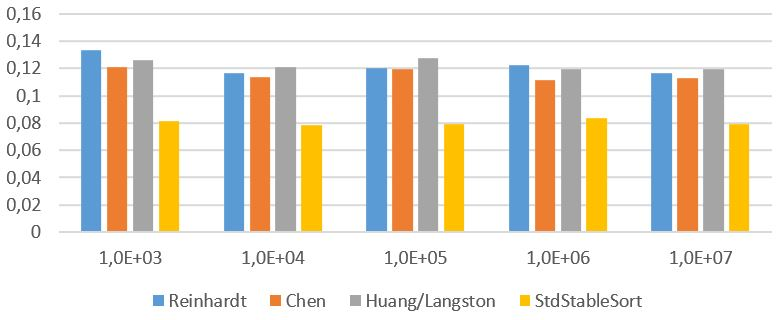
\includegraphics[width=\linewidth]{Diagramm-Bilder/big-beidesTeuer.JPG} \\
\caption{ $ \frac{Time}{n*log(n)} $ for different Bigtype list sizes $ n $ } \label{fig:big-beides-Teuer}
\end{figure}
The second result is mainly influenced by the number of comparisons and assignments (see below). As one can see, the used algorithm or version of algorithm should be chosen depending on the type for better performance. For a universal measure, independent of type, compiler and operating system, the number of comparisons and assignments can be evaluated. \\
\begin{figure}[H]
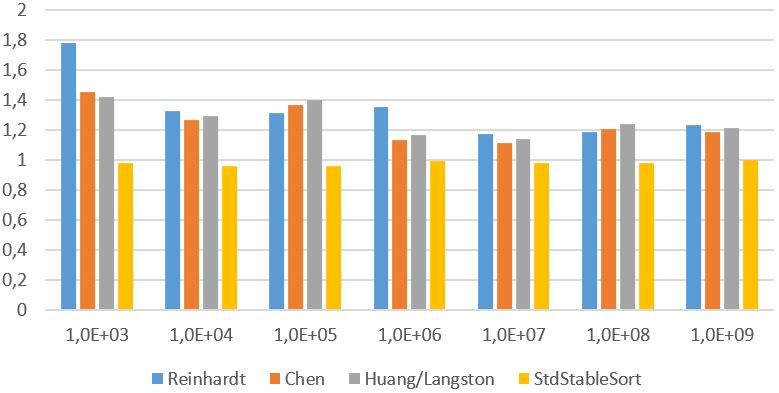
\includegraphics[width=\linewidth]{Diagramm-Bilder/ints-comparisons.JPG} \\
\caption{ $ \frac{Comparisons}{n*log(n)} $ for different list sizes $ n $ } \label{fig:ints-comp}
\end{figure}
\begin{figure}[H]
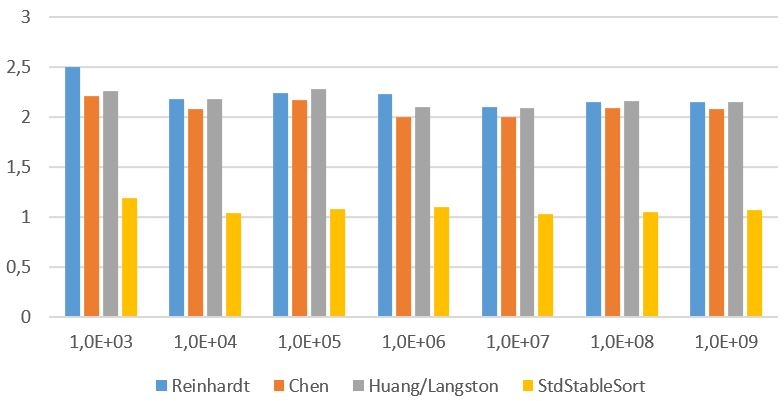
\includegraphics[width=\linewidth]{Diagramm-Bilder/ints-assignments.JPG} \\
\caption{ $ \frac{Assignments}{n*log(n)} $ for different list sizes $ n $ } \label{fig:ints-assign}
\end{figure}
The standard merge sort does roughly one assignment after one comparison and has only a small additional number of assignments (see result extra file). One can see that all our in-place versions need roughly just two assignments per comparison. \\
In a lot of diagrams, we show the results divided by n*log(n). Therefore, time, comparisons and assignments should be nearly constant throughout different list sizes for all mergesort implementations. To conclude to other specific implications, another scale may be used. E.g. the following diagram can be used as prove that the number of comparisons does not exceed 1.3n*log(n) + O(n). If this number is not exceed then the values do not increase for an increasing list size. \\
\begin{figure}[H]
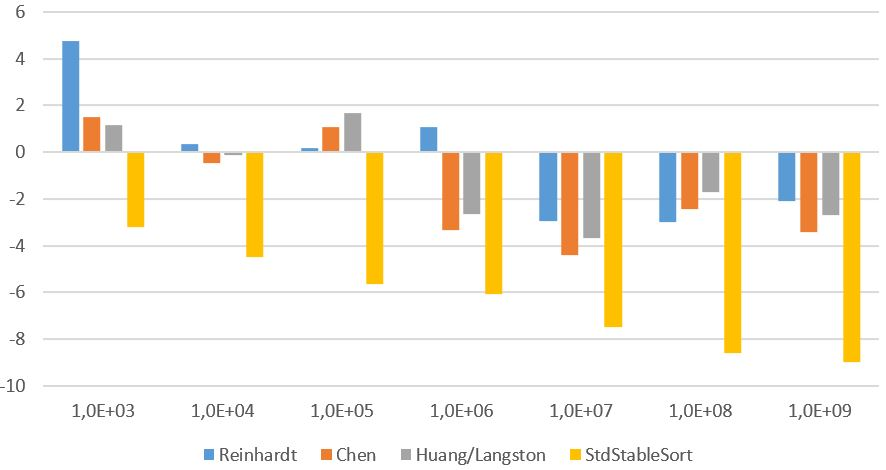
\includegraphics[width=\linewidth]{Diagramm-Bilder/ints-time-otherNormalization.JPG} \\
\caption{TODO: Comparisons with another normalisation} \label{fig:ints-time-otherNormalization}
\end{figure}
Although diagrams with n*log(n) instead of 1.3*nlog(n) also do not show a clear increase, it is impossible to use this diagram as a prove because of the fluctuating values in this case. \\
For a clearer comparison of Huang and Chen it is possible to just compare the merges because they can be substituted in the algorithm (results see extra file). But here it is important to mention that Reinhardt’s merge works completely differently because it merges to another range and though the std-inplace-merge merges to the same range, it needs additional memory to just make use of n-1 comparisons. \\
The runtime of the merges reflects the bad result of Chen in the first test more powerful. But it is important to remind that the runtime also depends on compiler and device. For a usual laptop and another compiler we got the following time average for multiple runs with 10 Mio elements (in the same test!): \\
\scriptsize
\begin{tabular}{|c|c|c|c|} \hline
Chen & Reinhardt & Huang & StdInpl-merge \\ \hline
148 418 ns & 88 717 ns & 99 766 ns & 147 056 ns \\ \hline
\end{tabular}
\normalsize \\
And if we make comparisons/assignments more relevant by use of lists with 1 million bigtype<30>, we get an entirely different relation of results for multiple runs on the laptop: \\
\scriptsize
\begin{tabular}{|c|c|c|c|} \hline
Chen & Reinhardt & Huang & StdInpl-merge \\ \hline
317 783 ns & 309 832 ns & 485 642 ns & 247 364 ns \\ \hline
\end{tabular}
\normalsize \\
In the above tests, we run the in-place algorithm of Reinhardt by using insertion sort in "reinhardt\_gapsort" for small cases and the asymmetric merge in "reinhardt\_merge". Furthermore we executed the quickselect step in every iteration. \\
But if we make specific demands to the sort, e.g. a small number of comparisons, we can switch to a more suitable mode. In the following, we will compare the different Reinhardt modes between themselves. In all runs, we use integer as type to be sorted. \\
\begin{figure}[H]
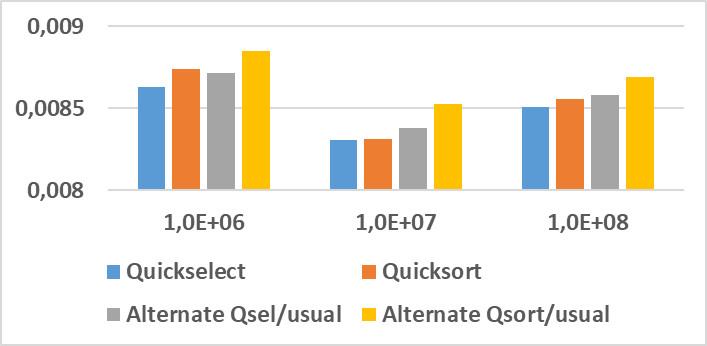
\includegraphics[width=\linewidth]{Diagramm-Bilder/diff-iterations-time.JPG} \\
\caption{ $ \frac{Time}{n*log(n)} $ different different Reinhardt itterations } \label{fig:diff-iterations-time}
\end{figure}
We can see that Reinhardt’s algorithm is fastest for integers if we just execute quickselect or quicksort iterations. Though these iterations need a bit more comparions for the execution of quicksort or quickselect, the number of assignments is smaller. This clearly can also be seen in the two following diagrams. \\
\begin{figure}[H]
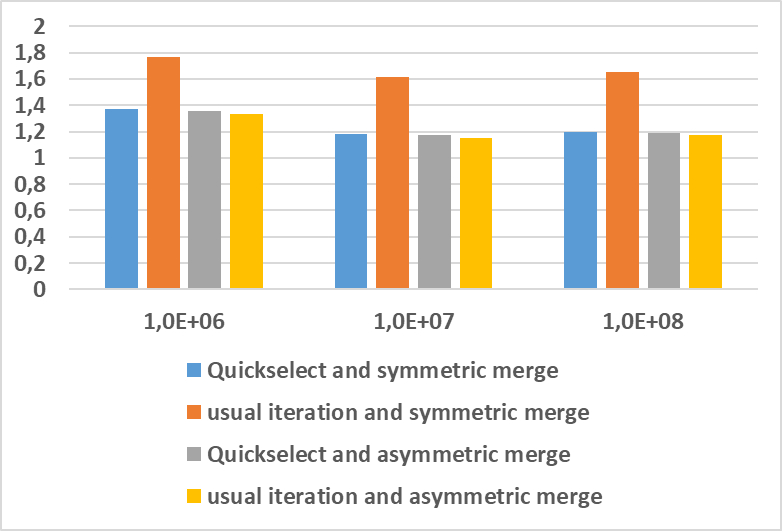
\includegraphics[width=\linewidth]{Diagramm-Bilder/diff-iterationsAndMerges-comparisons.JPG} \\
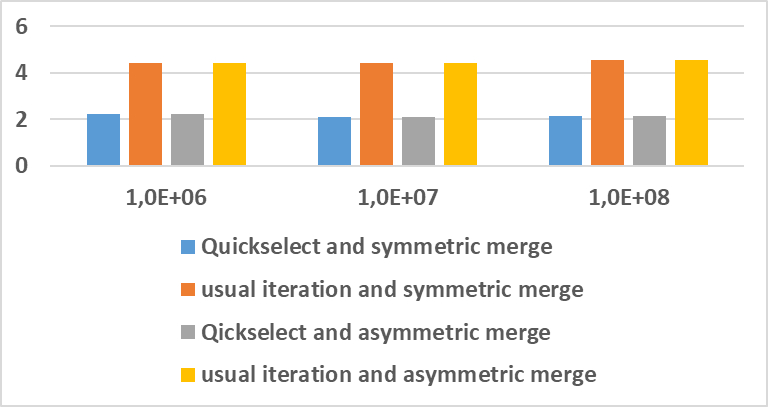
\includegraphics[width=\linewidth]{Diagramm-Bilder/diff-iterationsAndMerges-assignments.JPG} \\
\caption{Comparisons and Assignments for different Reinhardt merges} \label{fig:diff-iterationsAndMerges-assignAndComp}
\end{figure}
Merging asymmetric is a big improvement for time and number of comparisons (obviously not for number of assignments) of the usual iteration because in the usual iteration, the short list is always merged with all other sorted elements. For the time of the quickselect iteration, the asymmetric merge is, especially for the runtime, no improvement in this test case. \\
For a further reduction of comparisons and in the case of sorting bigtypes, it is also a good idea to replace insertion sort in the sort of the gap for small cases (here all along 50 elements) by aborting the recursive procedure later (3-smallsort). \\
\begin{figure}[H]
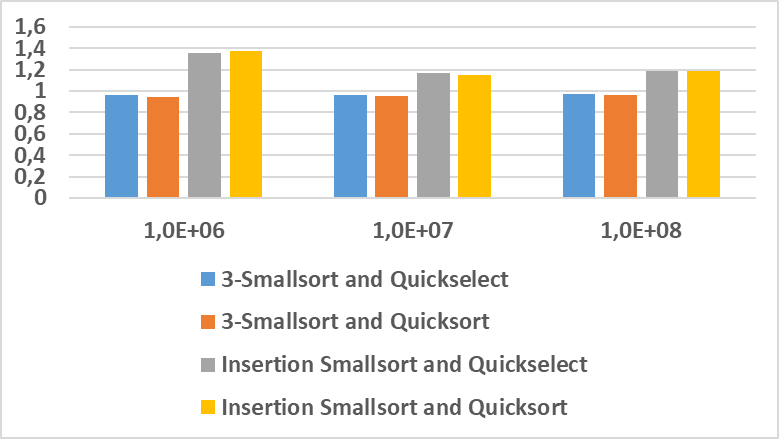
\includegraphics[width=\linewidth]{Diagramm-Bilder/comparisons-diff-iter-and-smallsorts.JPG} \\
\caption{Comparisons for different Reinhardt smallsorts} \label{fig:comparisons-diff-iter-and-smallsorts}
\end{figure}
The result is not surprising because merge sort needs less comparisons than insertion sort. But on the other side, insertion sort is used many times as sort for small cases because it is often executed faster for integers. \\
\begin{figure}[H]
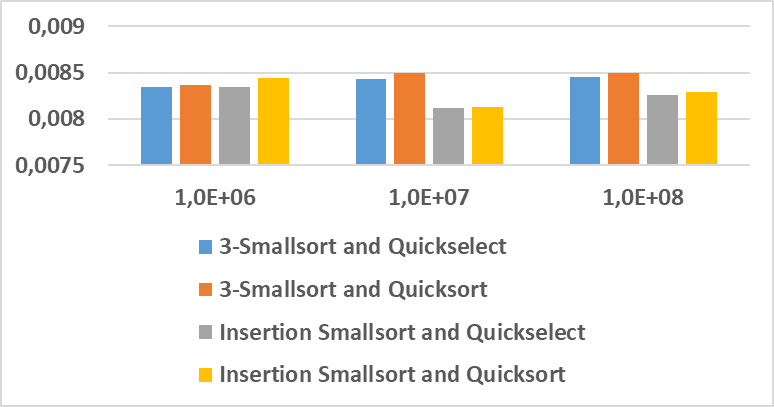
\includegraphics[width=\linewidth]{Diagramm-Bilder/time-diff-iter-and-smallsorts.JPG} \\
\caption{Time for different Reinhardt smallsorts} \label{fig:time-diff-iter-and-smallsorts}
\end{figure}
We also compared our implementations with some existing in-place merge sorts. \\
\begin{figure}[H]
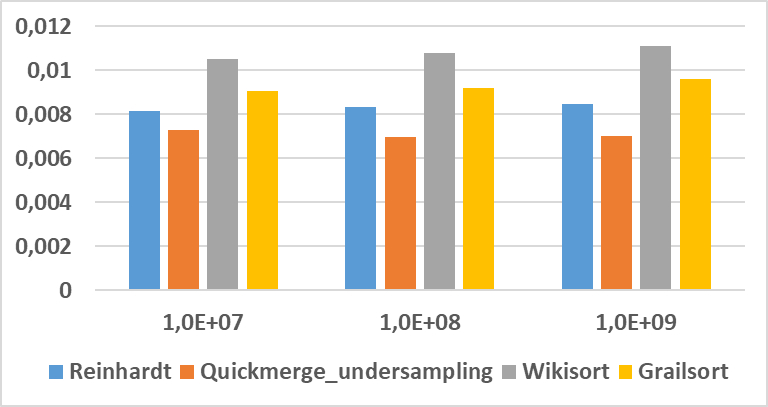
\includegraphics[width=\linewidth]{Diagramm-Bilder/time-other-inplace.JPG} \\
\caption{Time comparison with other inplace merge sorts} \label{fig:time-other-inplace}
\end{figure}
In terms of comparisons and moves they are able to compete with the other algorithms. It must be said that some more sophisticated and specialized implementations can slightly outperform our implementations when it comes to the measured time.

\bibliographystyle{amsplain}
\bibliography{sort}

\end{document}

